\documentclass{article}
\usepackage[utf8]{inputenc}
\usepackage{geometry}
\usepackage{graphicx}
\usepackage{pgfplots}
\usepackage{amsmath}
\usepackage{amssymb}
\usepackage{amsfonts}
\usepackage{mdframed}
\usepackage{amsthm}
\usepackage{tikz}
\usepackage{multicol}

\geometry{a4paper, left=2cm, right=2cm, top=1cm, bottom=2cm}

\pgfplotsset{compat=1.18}
\begin{document}

\begin{minipage}{0.7\textwidth}
    \small \textbf{LABORATORIO DE MECÁNICA VECTORIAL}  \\
    \small {Facultad de Ciencias, Universidad Nacional Autónoma de México} \\
    \small {Profesor: Radamés Ricardo Reynoso Manríquez} \\
    \small {Ayudante: Ana Laura Córdova Lara}\\
    \small {Fecha de entrega: 22 de Febrero de 2024} \\
    \small {Nombre completo: Andrés López González} \\
    \small {Tarea número III}
\end{minipage}
\hfill
\begin{minipage}{0.12\textwidth}
    
\includegraphics[width=\linewidth]{logo_universidad}
\end{minipage}

\section*{Cuestionario II}

PREGUNTA 1. Defina reproducibilidad de resultados de una medición, y patrón de referencia. \\\\
La reproducibilidad de resultados de una medición se refiere a la capacidad de obtener resultados consistentes y similares al repetir una misma medición bajo condiciones idénticas o muy similares. Esto implica que, si se repite la medición varias veces, los resultados deberían ser cercanos entre sí; esto está relacionado a lo visto al abarcar precisión y exactitud de la medida, pues para la reproductibilidad de resultados necesitamos que todos muestren un grado de dispersión muy bajo además de pertenecer a un intervalo delta en el que se halle la medición exacta real.\\\\

En el caso de un gas con un pistón en un proceso isotérmico, como un proceso isocórico (a volumen constante), la reproducibilidad se evidencia en la capacidad de obtener consistentemente la misma presión al mantener constante el volumen y la temperatura. Por ejemplo, si se mide la presión de un gas en un recipiente cerrado dígase Neón (que realmente desconozco si sea viable esta práctica) con un pistón fijo en una cierta temperatura y se repite este proceso varias veces, los valores de presión obtenidos deberían ser similares dentro de un margen aceptable de variación.\\\\

Por otro lado, un patrón de referencia es un estándar establecido y reconocido que se utiliza como punto de comparación para medir diversas magnitudes físicas. Estos patrones son fundamentales para asegurar la precisión y la consistencia en las mediciones realizadas en el laboratorio. Por ejemplo, el patrón internacional de tiempo es el segundo, lo cual veremos más adelante, definido por la vibración de un átomo de cesio 133; los patrones proporcionan una base confiable para realizar mediciones precisas y comparar resultados en diferentes experimentos y contextos científicos, así como la calibración de equipo de laboratorio como es el caso de una báscula.\\
En ocasiones no es tan formal como eso y de hecho para el kilogramo como ejemplo, hace tiempo se usaba como medida un objeto de justamente 1kg que era la unidad que se empleaba para referencia en aquel entonces, para equipo como básculas de fruterías muchas veces se hace algo similar y se busca algo que sea aproximado al kilogramo, aún si la incertidumbre es algo grande.
\\\\

PREGUNTA 2. En la tabla siguiente, se muestran los datos obtenidos de una resistencia eléctrica en función de la temperature de una bobina de cobre.
\begin{figure}[h]
  \centering
  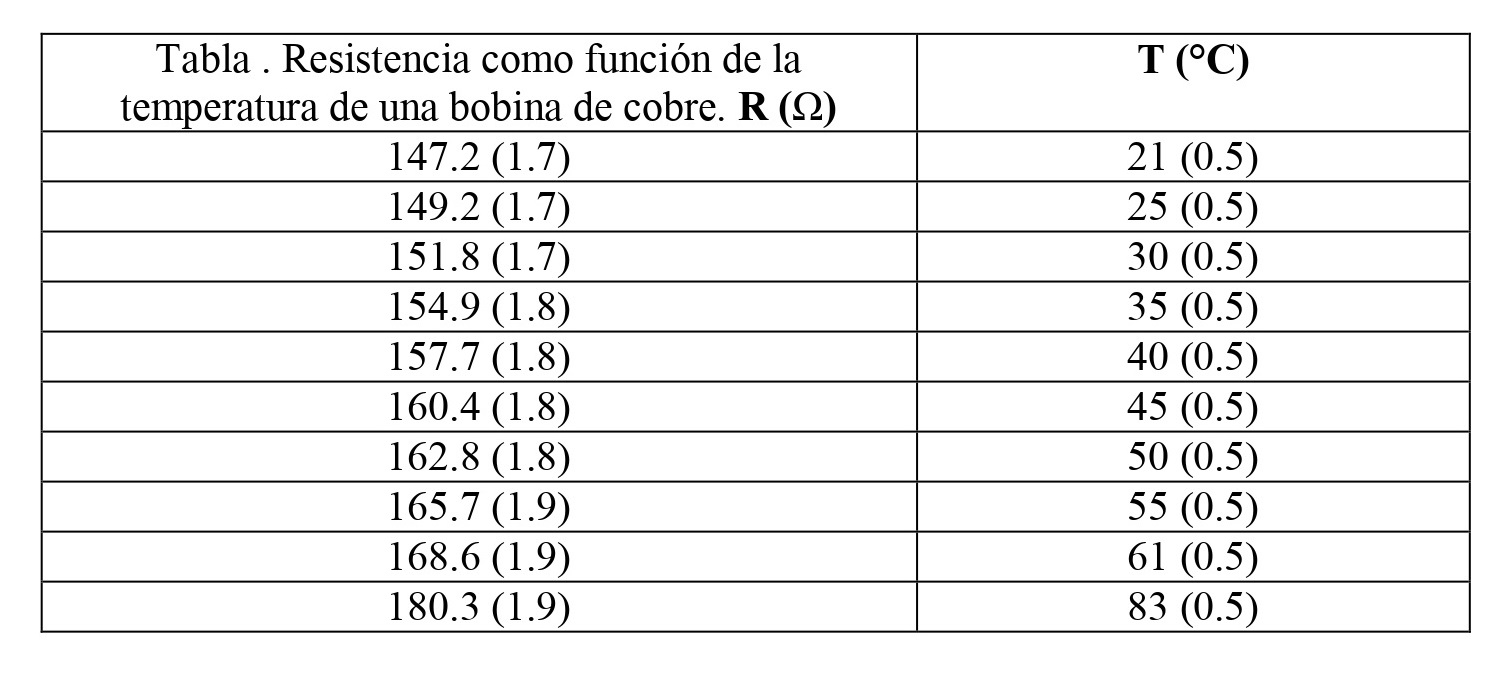
\includegraphics{enunc.jpg}
  \label{fig:enunc}
\end{figure}

\newpage
\begin{align*}
    \sum_{i=1}^n x_i &= [21 + 25 + 30 + 35 + 40 + 45 + 50 + 55 + 61 + 83 ]^{\circ}C = 445.0^{\circ}C \\
    \sum_{i=1}^n x^2_i &= [21^2 + 25^2 + 30^2 + 35^2 + 40^2 + 45^2 + 50^2 + 55^2 + 61^2 + 83^2 ] ^{\circ}C^2 = 22,951.0 ^{\circ}C^2 \\
    \sum_{i=1}^n y_i &= [147.2 + 149.2 + 151.8 + 154.9 + 157.7 + 160.4 + 162.8 + 165.7 + 168.6 + 180.3]\Omega = 1,598.6 \Omega \\
    \sum_{i=1}^n x_iy_i &= [(21 \cdot 147.2) + (25 \cdot 149.2) + (30 \cdot 151.8) + (35 \cdot 154.9) + (40 \cdot 157.7) + (45 \cdot 160.4) + (50 \cdot 162.8) \\ + (55 &\cdot 165.7) + (61 \cdot 168.6) + (83 \cdot 180.3)]\omega^{\circ}C = 72,825.7 \Omega^{\circ}C \\
\end{align*}
\textit{Calculemos la mejor recta ajustada utilizando lo visto en clase.}\\
\begin{align*}
    m &= \frac{E}{D} = \frac{(\sum_{i=1}^n x_iy_i) - n\Bar{X}\Bar{Y}}{(\sum_{i=1}^n x^2_i) - n\Bar{X}^2} = \frac{(\sum_{i=1}^n x_iy_i) - n(n^{-1}\sum_{i=1}^n x_i)(n^{-1}\sum_{i=1}^n y_i)}{(\sum_{i=1}^n x^2_i) - n(n^{-1}\sum_{i=1}^n x_i)^2} = \frac{72,825.7 - 10^{-1}(445.0)(1,598.6)}{(22,951.0)-10^{-1}(445.0)^2}\\
    &\approx 0.5361283150707 \\
    c &= \Bar{Y} - m\Bar{X} = (n^{-1}\sum_{i=1}^n y_i) - m(n^{-1}\sum_{i=1}^n x_i) \approx (10^{-1}\cdot1,598.6) - 0.5361283150707(10^{-1}(445.0)) \approx 136.00266 \\
    S_y &= \sum_{i=1}^n (Y_i-mX_i-c)^2 \approx \sum_{i=1}^n ((147.2)-0.53612(21)-136.00266)^2 \approx ((149.2)-0.53612(25)-136.00266)^2 \\ + ((151.8) &-0.53612(30) -136.00266)^2 + ((154.9)-0.53612(35)-136.00266)^2 + ((157.7)-0.53612(40)-136.00266)^2 \\
    + ((160.4) &-0.53612(45) -136.00266)^2 +((162.8)-0.53612(50)-136.00266)^2 + ((165.7)-0.53612(55)-136.00266)^2 \\
    + ((168.6) &-0.53612(61) -136.00266)^2 + ((180.3)-0.53612(83)-136.00266)^2 \approx 0.375661386
\end{align*}
\textit{I. Obténgase la incertidumbre de la pendiente}
\begin{align*}
    S_m &= S_y \sqrt{\frac{n}{n(\sum_{i=1}^n x^2_i) - (\sum_{i=1}^n x_i)^2}} \approx 0.375661386\sqrt{\frac{10}{10(22,951.0) - 445.0^2}} \approx 0.00669
\end{align*}
\textit{II. Obténgase la incertidumbre en la ordenada al origen}
\begin{align*}
    S_b &= S_y \sqrt{\frac{\sum_{i=1}^n x^2_i}{n(\sum_{i=1}^n x^2_i) - (\sum_{i=1}^n x_i)^2}} \approx 0.375661386 \sqrt{\frac{22,951.0}{10(22,951.0) - 445.0^2}} \approx 0.32073
\end{align*}
\textit{A continuación las siguientes imágenes (Figure 1, Figure 2) representan los valores dependientes e independientes proporcionados por la tabla, en donde el eje de las abscisas corresponde a la temperatura y el ordenado a la resistencia. Nótese que se marcó una franja, esta corresponde al intervalo medido teóricamente de incertidumbre en la medida, aunque podemos notar que por ocupar el método de mínimos cuadrados para la ecuación de la recta de la forma $f(x) = mx + c$ la incertidumbre se ha quedado enorme para la alta precisión que tuvo nuestra regresión lineal.}
\newpage
\textit{}\\\\\\
\begin{figure} [h]
    \centering
    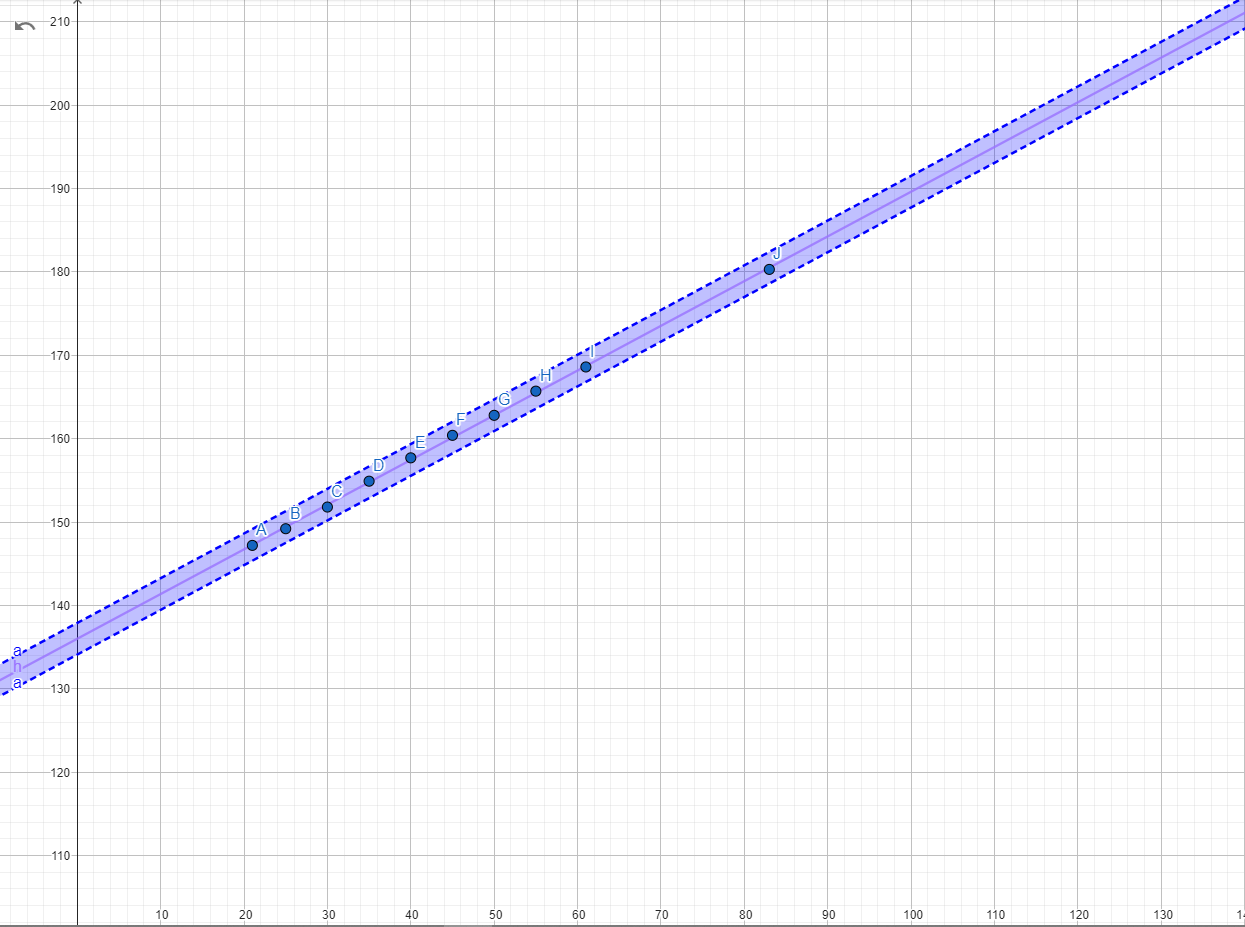
\includegraphics[width=0.74\linewidth]{Recta ajustada.png}
    \caption{Recta ajustada e intervalo de incertidumbre en $y_i$ asociado en la tabla.}
    \label{fig:enter-label}
\end{figure}
\textit{}\\\\\textit{}
\begin{figure} [h]
    \centering
    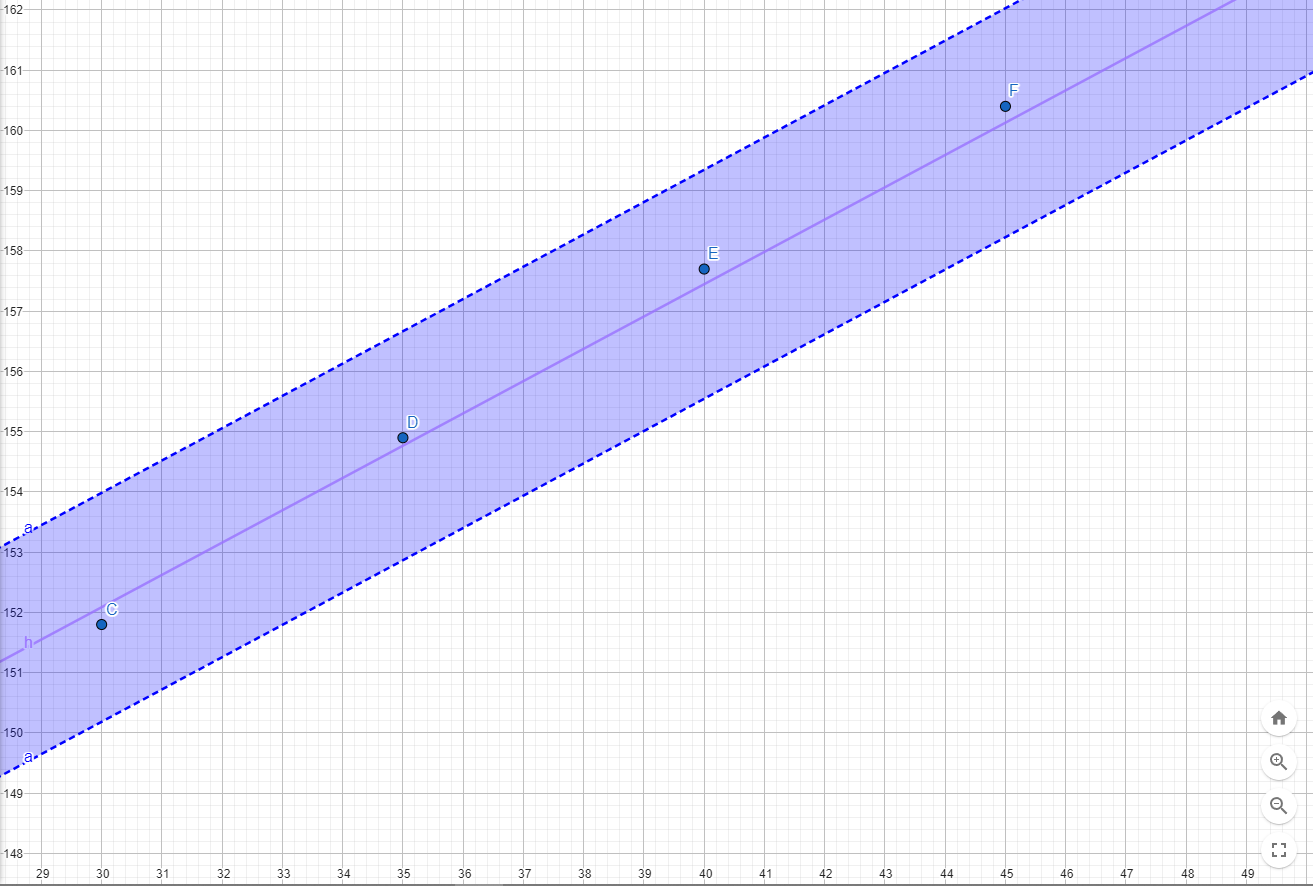
\includegraphics[width=0.74\linewidth]{Recta ajustada max.png}
    \caption{Misma recta amplificada para vista de la dispersión respecto a mi ecuación (ínfima).}
    \label{fig:enter-label}
\end{figure}
\newpage

PREGUNTA 3.  Defina los patrones de referencia más actuales para: Segundo, kilogramo, metro, e intensidad luminosa.\\\\
\textit{El segundo se define actualmente en función de las oscilaciones causadas por la radiación electromagnética de un átomo de cesio 133, un isótopo de este. Un segundo se define como lo que tardan 9,192,631,770 períodos de la radiación correspondiente a la transición entre los dos niveles hiperfinos del estado fundamental del átomo de cesio-133.}\\

\textit{El kilogramo en cambio se mide de una forma muy distinta, en realidad cada unidad de medida tiene formas muy peculiares de "definirse", se define en términos de la constante de Planck (h) mediante el experimento conocido como balanza de Watt. Desde la revisión de la definición en 2019, el kilogramo se define exactamente como la masa que posee un objeto cuando la frecuencia de su vibración es de exactamente de 1,356,392,512 hertzios.}\\

\textit{ El metro se define como la longitud del trayecto recorrido por la luz en el vacío durante un intervalo de tiempo de 1/299,792,458 de segundo. Esto viene de la implicación que la velocidad de la luz en el vacío se define exactamente como 299,792,458 metros sobre segundo, con lo que resulta hasta trivial cuánto tarda la luz en esa fracción de segundo (1m).}\\

\textit{Finalmente la unidad de intensidad luminosa es la candela (que es diferente a los lúmenes). Se define en términos de la radiación emitida por una fuente de luz muy específica. Se obtiene en términos de la intensidad luminosa emitida por una fuente monocromática de frecuencia $540 × 10^12$ hercios con una potencia radiante de 1/683 vatios por estereorradián.}\\\\\\



PREGUNTA 4. Para determinar el volumen de un prisma rectangular se mide la longitud de los lados y se obtiene como resultado: Largo (5.1 + 0.1) cm, ancho (3.25 + 0.05) cm, y alto (10.0 + 0.1) cm.\\
a) ¿Cuáles son las cifras significativas respectivas del mesurando de las mediciones?\\
\textit{El primer mesurando tiene 2 cifras significativas (1 entera, 1 decimal), el segundo de ellos tiene 3 cifras significativas (1 entero, 2 decimales), el último también tiene 3 cifras significativas pero de distinta forma (2 enteras, una decimal). Es interesante resaltar que la incertidumbre del tercero también tiene 3 cifras significativas implícitamente pues es en realidad es 00.1 por venir del mesurando principal $xx.x$, no obstante esto no es algo convencionalmente aceptado por lo que se redacta 0.1.}
b) ¿Cuál es el volumen de este prisma rectangular, considerando las cifras significativas apropiadas?
\textit{Considérese la fórmula del volumen de un prisma como una función multivariable.}
\[ f:\mathbb{R}^3 \Rightarrow \mathbb{R} \quad f(a,l,h) = V = \bar{a}\bar{l}\bar{h} \]
\[ \Delta_{abs} = \| \frac{\partial v}{\partial a} \| \Delta a + \| \frac{\partial v}{\partial l} \| \Delta l + \| \frac{\partial v}{\partial h} \| \Delta h = \| \bar{l}\bar{h} \| \Delta a + \| \bar{a}\bar{h} \| \Delta l + \| \bar{a}\bar{l} \| \Delta h \] 
\[ = [(5.1)(10.0)(0.05) + (3.25)(10.0)(0.1) + (3.25)(5.1)(0.1)]cm^3 = 7.4575cm^3 \]
\[ V_{med} = a_{med}l_{med}h_{med} = (5.1)(3.25)(10.0)cm^3 = 165.75cm^3 \]
\[ V_{real} = 165.75cm^3 \pm 7.4575cm^3 \]
\newpage
PREGUNTA 5. Después de realizar un experimento de Movimiento Uniforme Acelerado, se obtuvieron los resultados que se muestran en la Tabla 1. El procedimiento consistió en medir tres veces los tiempos necesarios para que un móvil se desplazara de una posición inicial $x = 0 m$, hasta las posiciones finales $x_f$ que se muestran en la primer columna de la Tabla 1. El reloj usado para medir el tiempo, asocia al resultado de la medición una incertidumbre de $\pm 0.001 s$.
\begin{figure}[h]
\centering
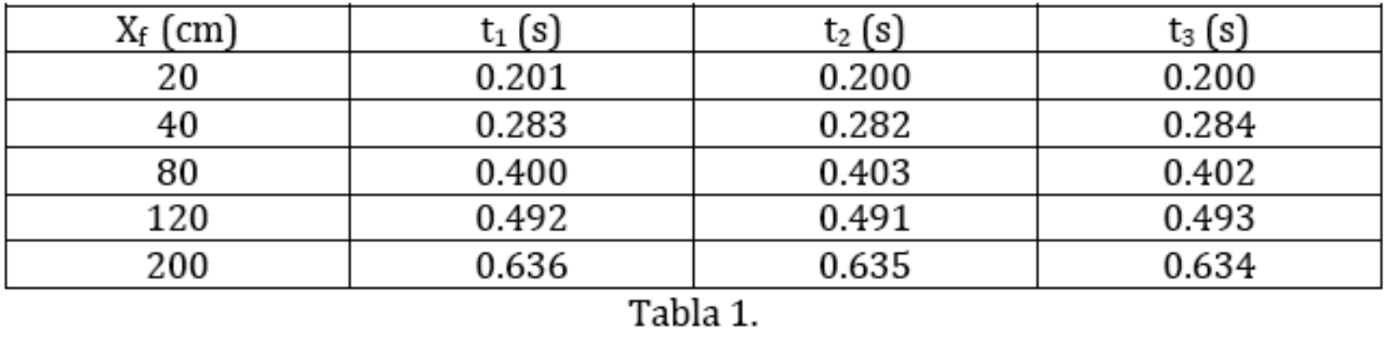
\includegraphics[width=0.61\textwidth]{table.png}
\label{fig:tabla}
\end{figure}
De acuerdo a la información anterior determine:\\
a) El valor más representativo de los tres tiempos medidos para cada desplazamiento.\\
\textit{En $x_f=20cm$ el valor más representativo de los tres es 0.200, en $x_f=40cm$ es 0.283, en $x_f=80cm$ 0.402, en $x_f=120cm$ es 0.492 y finalmente en $x_f=200cm$ es 0.635; el criterio con el que escogí estos valores es en términos coloquiales la mediana de un conjunto de 3 datos... en términos más analíticos, estos al estar en medio de los dos extremos nos proporcionan una región de incertidumbre de radio $\pm 0.001s$ que será más precisa si fijamos el centro de nuestro disco cerrado en este valor central, de modo que por ejemplo en $x_f=40cm$ centrar nuestro disco cerrado en 0.283 nos dará que el valor real llámese x estará centrado en $y_0=0.283s$ y estará en una región cerrada de radio 0.001s: $x \in [y_0-\delta, y_0+delta] \, \implies \, x \in [0.283-0.001, 0.283+0.001] : [x] = segundos$. Lo cual finalmente es $x \in [0.282, 0.284] : [x] = segundos$ lo que corresponde con la realidad.}\\\\
b) El valor medio de los tres tiempos para cada desplazamiento. \\
\textit{El valor medio de un conjunto de datos se define como $n^{-1}\sum_{i=1}^n x_i$.}
\begin{align*}
    x_f = 20cm &\implies \bar{x} = \frac{0.201+0.200+0.200}{3}s \approx 0.20033s \cong 0.200s \\
    x_f = 40cm &\implies \bar{x} = \frac{0.282+0.283+0.284}{3}s = 0.283s \\
    x_f = 80cm &\implies \bar{x} = \frac{0.400+0.402+0.403}{3}s \approx 0.40166s \cong 0.402s \\
    x_f = 120cm &\implies \bar{x} = \frac{0.492+0.491+0.493}{3}s = 0.402s \\
    x_f = 200cm &\implies \bar{x} = \frac{0.636+0.635+0.634}{3}s = 0.635s \\
\end{align*}

\end{document}
